%=====================================================
%====== If you are new to LaTeX, this website ========
%======     will be your new best friend:     ========
%======   http://en.wikibooks.org/wiki/LaTeX  ========
%======   Template created by Jonathan Blair  ========
%=====================================================



%=====================================================
%============ Controls ===============================
%=====================================================

%\documentclass[12pt,letterpaper,onecolumn]{article}
\documentclass[11pt,letterpaper,onecolumn]{article}
%\documentclass[10pt,letterpaper,onecolumn]{article}  % not recommended
%\documentclass[12pt,letterpaper,twocolumn]{article}
%\documentclass[11pt,letterpaper,twocolumn]{article}
%\documentclass[10pt,letterpaper,twocolumn]{article}


\usepackage{amsmath}
\usepackage{graphicx}
\usepackage{url}
\usepackage{textgreek}
\usepackage{float}
%\graphicspath{{path-to-folder-containing-necessary-graphics}{other folder as necessary}}


%=====================================================
%============ \begin{document} =======================
%=====================================================

\begin{document}

%=====================================================
%============ Title ==================================
%=====================================================

\title{\bf Use of Electron Diffraction to Determine the Crystal Spacing in Graphite}
%\title{\Large\bf Larger, Bolded Title}

%=====================================================
%============ Author =================================
%=====================================================
\author{
 Jairo Portillo \\*
  \\*
 PHY 353L Modern Laboratory \\*
 Department of Physics \\*
 The University of Texas at Austin \\*
 Austin, TX 78712, USA
}
\date{October 12, 2015}

%\address{The University of Texas, Austin, Texas, 78712}

\maketitle

%=====================================================
%============ Abstract ===============================
%=====================================================

\begin{abstract}

An electron beam was fired at a graphite sample in order to generate a diffraction pattern. This diffraction pattern will allow the determination of the wave nature of electrons. We used the De Broglie hypothesis and Bragg's law to determine the first order crystal spacing of graphite coated Nickel mesh. We found $d_{1}$ = 3.053$\pm$0.0453 $\AA$ and $d_{2}$ = 1.586$\pm$0.0146 $\AA$, which give a ratio of .519$\pm$.004. Our ratio is 1.9$\%$ from the accepted ratio of 0.577.

\end{abstract}

%=====================================================
%============ Body of the article ==========================
%=====================================================

%=====================================================
%============ Section ==================================
%=====================================================

\section{Introduction}

\subsection{Physics Motivation}

The dual nature of light had been an unfamiliar phenomenon until Einstein proposed the idea of the photon. Louis de Broglie hypothesized that just as radiation has particle-like properties, then electrons and other particles could possess wave-like properties. He assumed that the wavelength of the electrons had to be inversely proportional to its momentum. We will confirm de Broglie's hypothesis by firing electrons at a graphite coated nickel mesh in an Electron Diffraction Tube. The crystal structure of graphite behaves as a grating for the electrons producing a diffraction pattern, demonstrating the electron's wave nature.With Bragg's law the spacing of the graphite can be determined from the wavelength of the electron and the angle the electron diffracted off of the graphite.~\cite{Bas,Nave} 

\subsection{Theoretical background}

De Broglie proposed that the wavelength of a particle can be found by:
$$\lambda = \frac{h}{p}$$
where h is Plank's constant, and p is the momentum. To give the electrons momentum, they pass through a potential difference or an accelerating voltage $V_a$. The momentum can be found by setting the kinetic energy $K=\frac{1}{2}mv^2$ with the potential energy $U=eV_a$ yielding:
$$p = \sqrt{2m_{e}eV_{a}}$$
where $V_{a}$ is the acceleration voltage, e is the charge of an electron and $m_{e}$ is the mass of the electron.The angle of incidence $\theta$ is related to the wavelength $\lambda$ through Bragg's law: 
$$2d\sin{\theta}=n\lambda$$
Bragg's law describes the position of interference maxima, where d is the atomic spacing of the graphite and n is the order of the reflection. By substituting the wavelength $\lambda$ into Bragg's law give a linear relationship between the aangle of incidence and the accelorating voltage
$$sin(\theta)=\frac{1}{2d}\frac{hn}{\sqrt{2m_{e}eV_{a}}}$$
This relationship will be used to calculate the atomic spacing for each of the rings.

\subsection{Crystal Spacing}

\begin{figure}[H]
  %
  % placement specifier = { h,t,b,p,!,H }
  % see the following url for placement specifier definitions:
  % http://en.wikibooks.org/wiki/LaTeX/Floats,_Figures_and_Captions
  %
 \begin{center}
 \includegraphics*[scale = 0.5]{GeoStructure.jpg}
  %
  %               [llx,lly][urx,ury]{ filename.eps }
  %
  % Note: llx = lower left x coordinate
  %       lly = lower left y coordinate
  %       urx = upper right x coordinate
  %       ury = upper right y coordinate
  %
  %       If [ llx,lly ] is omitted, [0,0] is assumed.
  %       Be sure to include units.
  %
 \caption{Diagram of the (002) plane of graphite\label{fig:struct}}
 % See http://en.wikibooks.org/wiki/LaTeX/Labels_and_Cross-referencing
 %  for information on labels.
 \end{center}
\end{figure}

Graphite has a hexagonal structure, which could create a diffraction patter of six rings. However, the rings superpose. This is dues to the weak inter-plane bonding which results in each plane being randomly oriented to the other. This gives one ring for $d_1$ and $d_2$ rather than six each. The ratio of the atomic spacings come from the ratio of the miller indicies with $d_1$ being the (110) plane and $d_2$ the (100) plane which gives $\frac{1}{\sqrt{3}}$.~\cite{EDF,UM}



%=====================================================
%============ Section ==================================
%=====================================================

\section{Experimental setup}



\subsection{Apparatus}

\begin{figure}[H]
  %
  % placement specifier = { h,t,b,p,!,H }
  % see the following url for placement specifier definitions:
  % http://en.wikibooks.org/wiki/LaTeX/Floats,_Figures_and_Captions
  %
 \begin{center}
 \includegraphics*[scale = .5]{Lab2.png}
  %
  %               [llx,lly][urx,ury]{ filename.eps }
  %
  % Note: llx = lower left x coordinate
  %       lly = lower left y coordinate
  %       urx = upper right x coordinate
  %       ury = upper right y coordinate
  %
  %       If [ llx,lly ] is omitted, [0,0] is assumed.
  %       Be sure to include units.
  %
 \caption{The Electron Diffraction Tube where: $V_f$ is the filament voltage (6.3V), $V_a$ is the accelerating voltage, $V_b$ is the bias voltage, C is the cathode, E is the electron beam, $F_1$ and $F_2$ are the focusing rings, A is the anode, and T is the target. \label{fig:EDT}}
 % See http://en.wikibooks.org/wiki/LaTeX/Labels_and_Cross-referencing
 %  for information on labels.
 \end{center}
\end{figure}


This experiment occurs within the vacuum of the Electron Diffraction Tube. The cathode is heated by the filament voltage $V_f$ which allows electrons to flow. The cathode is in a shield known as a cathode can which allows the control of the anode current and focuses the electron beam. The electrons are allowed to travel through the tube as there is an electric field between the cathode and anode. The accelerating voltage $V_a$ is the driving potential applied between the cathode and anode. When the electrons hit the film aafte rthe annode, the electrons diffract off the atoms the graphite developing the pattern.

The bias voltage $V_b$ was applied by a separate source and allowed the electron beam to be focused in order to make the diffraction pattern visible. The bias voltage maintains the cathode at a higher potential than the glass bulb so the electrons are kept away from the cathode. $V_f$ heats up the filament with 6.3V AC, which is kept constant throughout the experiment. The ammeter is attached in order to protect the filament from being damaged. The Electron Diffusion Tube can only maintain currents under about 15mA, anything higher will render it unusable.~\cite{ML}



%=====================================================
%============ Importing pictures  ==========================
%=====================================================

% !! To be imported, all graphics must be converted !!
% !!    to encapsulated postscript (.eps format)    !!
% !!  The GNU Image Manipulation Program (GIMP) is  !!
% !!          capable of this conversion.           !!



\subsection{Data Collection}

Since we were working with a high voltage apparatus, we had to make sure all the connections were secure and were aware of any fail safe the circuit may have to protect the film. One fail safe was to break the circuit between the ammeter and the tube. Another was to increase the bias voltage in order the prevent the flow of electrons rendering no pattern but protecting the film if the accelerating voltage gets too high.

We measured the rings with a plastic callipers. We took multiple measurements of the inner and outer diameter for each of the rings. With the multiple measurements error was calculated and an average diameter for each ring. The calculated error was more reasonable than the standard $\pm$0.05 mm error of the caliper as the fuzzy edges on the rings did not give definite measurements.

\begin{table}[H]
\centering
\begin{tabular}{|c|c|c|c|}
\hline
 Voltage (kV) & Average $D_1$ (mm) & Average $D_2$ (mm)\\
 Error: $\pm$.05 & Error: $\pm$1.78 & Error: $\pm$1.78 \\ \hline
 2.2 & 25.00 & 47.00 \\
 2.7 & 22.00 & 42.00 \\
 3.3 & 19.66 & 38.17 \\
 4.0 & 17.34 & 34.67 \\
 4.5 & 15.84 & 31.34 \\
 5.0 & 15.34 & 29.34 \\
 \hline
\end{tabular}
\caption{Our Data. $D_i$ are the diameters}
\label{tab:data}
\end{table}
%===================================================
%============ Section ==================================
%=====================================================

\section{Data Analysis and Results}

\subsection{Geometry}

\begin{figure}[H]
\centering
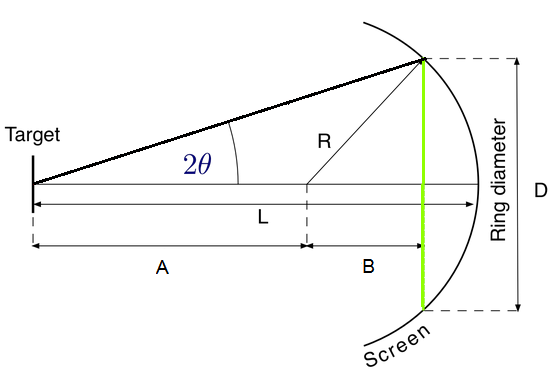
\includegraphics{GeometryTube.PNG}
\caption{Geometry of the diffraction pattern with respect to the angle of diffraction}
\label{fig:Geo}
\end{figure}

With some trigonometry, we can find the relationship between the diameters D and the angle of diffraction $\theta$ and the assumption that $\frac{D}{2}\approx R\alpha$, where $\alpha$ is the angle between R and B. L is the length of the path and R is the radius of the bulb. That relatonship is:
$$\theta=\frac{1}{2}\arctan{[\frac{R\sin{\frac{D}{2R}}}{L - R + R\cos{\frac{D}{2R}}}]}$$

\subsection{Data Processing and Hypothesis Testing}

As seen in Table~\ref{tab:data} we obtain diameters for each voltage. With these voltages, the wavelength could be found and a plot between $\sin{\theta}$ and wavelength $\lambda$.

\begin{table}[H]
\centering
\begin{tabular}{|c|c|}
 \hline
 Voltage(kV) & Wavelength(pm) \\
 Error: $\pm$.05 &  \\ \hline
 2.2 & 26.15$\pm$.59 \\
 2.7 & 23.60$\pm$.44 \\
 3.3 & 21.35$\pm$.32 \\
 4.0 & 19.39$\pm$.24 \\
 4.5 & 18.28$\pm$.20 \\
 5.0 & 17.35$\pm$.17 \\
 \hline
 
\end{tabular}
\caption{Voltage to Wavelength}
\label{tab:vtl}
\end{table}

%=====================================================
%============ Importing pictures  ====================
%=====================================================

% !! To be imported, all graphics must be converted !!
% !!    to encapsulated postscript (.eps format)    !!
% !!  The GNU Image Manipulation Program (GIMP) is  !!
% !!          capable of this conversion.           !!

\begin{figure}[H]
  %
  % placement specifier = { h,t,b,p,!,H }
  % see the following url for placement specifier definitions:
  % http://en.wikibooks.org/wiki/LaTeX/Floats,_Figures_and_Captions
  %
 \begin{center}
 \includegraphics*[scale = .6]{PlotED.pdf}
  %
  %               [llx,lly][urx,ury]{ filename.eps }
  %
  % Note: llx = lower left x coordinate
  %       lly = lower left y coordinate
  %       urx = upper right x coordinate
  %       ury = upper right y coordinate
  %
  %       If [ llx,lly ] is omitted, [0,0] is assumed.
  %       Be sure to include units.
  %
 \caption{ Plot of $\sin{\theta}$ vs wavelength $\lambda$.~\label{fig:results} }
 % See http://en.wikibooks.org/wiki/LaTeX/Labels_and_Cross-referencing
 %  for information on labels.
 \end{center}
\end{figure}

In Fig~\ref{fig:results}, the linear relationship between the wavelength and $\sin{\theta}$ are plotted. $d_1$ corresponds to the plot for inner diameters and $d_2$ corresponds to the plot for outer diameters. The linearity of the plot confirms de Broglie's hypothesis and the Bragg's law. This confirms the wave nature of the electron as it shows that it has a wavelength and exhibits wave behavior. The slope for $d_1$ was found to be 0.00163 $\pm$ 2.43E-5 and for $d_2$ was 0.00315 $\pm$ 2.91E-5. So for the actual atomic spacing $d_1$ is  305.34 $\pm$ 4.53 pm and $d_2$ is 158.58 $\pm$ 1.46 pm. The ratio of our $d_1$ and $d_2$ give .519$\pm$.004, which is 1.9$\%$ from the accepted ratio of 0.577. This ascertains that we observed the diffraction pattern of the (110) and (100) planes of graphite.

The error in our voltage measurements were the standard one half the smallest unit which was $\pm$.05 kV. Since we did not use a constant bias voltage throughout the experiment and did deem the standard error in the caliper suitable, the error of our diameter measurements is the deviation of the mean of our diameter measurements. The error in the angle and wavelength were found by finding the percent error in our measurements and multiplying it by our calculated values.

%===========================================================================
%=========================== Table 1 =======================================
%===========================================================================
%
% Note: the position of the table does not always depend on its position here. See
% http://en.wikibooks.org/wiki/LaTeX/Tables
% for details.
%

%=====================================================
%============ Section ==================================
%=====================================================

\section{Summary and conclusions}

The linearity of the plot of $\sin{\theta}$ against the wavelength $\lambda$, which is dependent on the accelerating voltage, confirms the de Broglie hypothesis and Bragg's law and thus electrons behaves as waves. With the slopes of both fits the atomic spacing of $d_1$ and $d_2$ was found to be 305.34 $\pm$ 4.53 pm and 158.58 $\pm$ 1.46 pm, respectively. The ratio of our $d_1$ and $d_2$ give .519$\pm$.004, which is 1.9$\%$ from the accepted ratio of 0.577, which confirms the geomatric structure of graphite.

%=====================================================
%============ Bibliography  ==============================
%=====================================================

\begin{thebibliography}{9}

\bibitem{Bas}	
Subhasish Basak, ``de Broglie’s hypothesis: wave-particle duality
," Retrieved 10/10/2015, \url{http://physics.niser.ac.in/~sbasak/p303_2010/06.08.pdf}. 

\bibitem{Nave}
Carl R. Nave, ''HyperPhysics: Davisson-Germer Experiment," Retreived 10/9/2015, \url{http://hyperphysics.phy-astr.gsu.edu/hbase/hph.html}.

\bibitem{ML}
 ''Electron Diffraction Lab," Retrieved 9/27/2015, \url{https://web2.ph.utexas.edu/~phy353l/lab/electron_diff/Electron_Diffraction.pdf}

\bibitem{EDF}
School of Physics at Georgia Tech, ''Electron Diffraction Experiment," Retrieved 10/10/2015, \url{http://advancedlab.physics.gatech.edu/labs/waveparticle/wave-particle-2.html}.

\bibitem{UM}
University of Michigan, ''Electron Diffraction and Crystal Structure," Retrieved 10/11/2015, \url{http://instructor.physics.lsa.umich.edu/adv-labs/Electron_Diffraction/electron_diffraction2.pdf}.

\end{thebibliography}

%=====================================================
%============ End ====================================
%=====================================================

\end{document}

%=====================================================
%============ End ====================================
%=====================================================
